% !Mode:: "TeX:UTF-8"
\chapter{相关原理与技术}

\section{程函方程}
程函方程是当使用WKB理论来近似波动方程时在波动传播问题中碰到的非线性偏微分方程。它从电磁学的麦克斯韦尔方程组导出,并在物理 (波动)光学和几何 (射线)光学之间起连接作用。

它的一般形式是:
\begin{equation}
    \label{eikonal_equation_1}
    \left| \nabla u(x) \right| = a(x), x \in \Omega
\end{equation}

约束条件是边界$u(x)$梯度为0。$a(x)$值为正。$\nabla$是梯度,$\left| \right|$是欧几里得范数。这里,右边的$a(x)$是已知的,物理上来说,$u(x)$的求解结果是边界运动到里面某个点$x$所需要的最短时间,此时$a(x)$表示在$x$上花费的时间。

一种快速计算程函方程近似解的方法就是快速行进法。当$a = 1$的特殊情况下,方程的解就是内部点到边界的有符号距离。

在2D情况下,我们求解程函方程,即下面的问题:
\begin{equation*}
    \label{eikonal_equation_2}
    \left\{
    \begin{aligned}
    \left| \nabla u \right| = a & \mbox{on} & \Omega \\
    u = 0 & \mbox{on} &  \partial\Omega
    \end{aligned}
    \right.
\end{equation*}

$\Omega$是平面里面的一个封闭物体。我们离散化变量$x$:$x_{I} = I\Delta x\mbox{其中}I = (I_{1}, I_{2}) \in Z_{2}, \Delta x > 0$。然后将
\begin{equation*}
    \label{eikonal_equation_3}
    \left| \nabla u(x) \right| - a(x) = 0
\end{equation*}

离散化为以下格式:
\begin{equation*}
    \label{scheme}
    S_{I}(\{u_{J}\}_{J \in V(I)}) = 0
\end{equation*}

其中,$V(I) = \{J \in Z^{2}, \left| J - I \right| \leq 1\}$,也就是说$V(I)$是点$I$在平面网格上的相邻5点(看)。于是我们有了
\begin{equation*}
    \label{eikonal_equation_3}
    V(I) = \{I, I^{1, +}, I^{1, -}, I^{2, +}, I^{2, -}\} \mbox{ 其中 } I^{\alpha, \pm}  = I \pm e_{\alpha}, \alpha = 1, 2
\end{equation*}

我们推荐Rouy-Tourin格式
\begin{equation}
    \label{eikonal_equation_3}
    \begin{aligned}
    & -a(x_I) + \sqrt{(\max(0, \frac{u_I - u_{I^{1, -}}}{\Delta x}, \frac{u_I - u_{I^{1, +}}}{\Delta x}))^2 + (\max(0, \frac{u_I - u_{I^{1, -}}}{\Delta x}, \frac{u_I - u_{I^{1, +}}}{\Delta x}))^2} \\
    & := S_I(u_I, u_{I^{1, -}}, u_{I^{1, +}}, u_{I^{2, -}}, u_{I^{2, +}}) := S_I[u]
    \end{aligned}
\end{equation}

\section{快速行进法}
快速行进法(Fast Marching Method, FMM)是由Sethian在1996年提出的,用来求解从已知边界向内部演化的过程。它以某种方式记录了物体边界向前行进的信息。
\begin{figure}[h!]
    \centering
    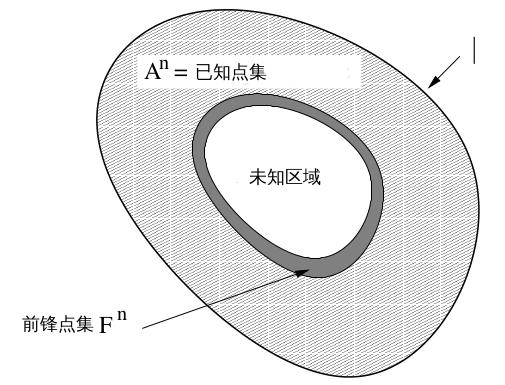
\includegraphics[width=300bp]{figure/sets_fmm.png}
    \caption{FMM的各个集合:已知点集$A^n$,前锋点集$F^n$和未知区域}
    \label{fig-sets_fmm}
\end{figure}

首先我们定义一个递增时间序列$(t_{n})_{n}$,其中$t_{0} = 0$,一个递增集合序列$(A^{n})_{n}$和一个非递增函数序列$(u^{n})_{n}$,其中,每一个$Z^{2}$网格上的点$I$都对应定义$u^{n} = (u^{n}_{I})_{I}$。$u^n$在$A^n$上面计算出来的值就是程函方程里$u$的解。这也是为什么$A^n$被称为已知点集,因为$u^n$与$A^n$外面的点没有关系,我们设置
\begin{equation*}
    \label{far_region}
    u^n_I = +\infty \mbox{当} I \in Z^2 \setminus A^n
\end{equation*}

另一方面,$t_n$的值是
\begin{equation*}
    \label{tn_in_fn}
    u^n_I = t_n \mbox{当} I \in A^2 \setminus A^{n-1}
\end{equation*}

即$t_n$是已知点集$A^n$中相对于$A^n$新增的点的一般值。

看图很容易就能想到,前锋点集$F^n$就是已知点集$A^n$的离散边界,就是说
\begin{equation*}
    \label{fn_1}
    F^n = \{ I \in Z^2 \setminus A^n, \mbox{所以} V(I)\cap A^n \neq \textrm \O \}
\end{equation*}

为了更方便的应用到FMM算法里面,我们改写上式为
\begin{equation*}
    \label{fn_2}
    F^n = ( \underset{I \in A^n}{\cup}V(I)) \setminus A^n
\end{equation*}

前锋点集$F^n$是在$A^n$外面,离$A^n$很近的一组网格点。所以我们又称前锋点集为“窄带”。我们将要在这个点集里面为$A^{n+1} \setminus A^n$寻找新的点,即
\begin{equation*}
    \label{fn_3}
    A^{n+1} \setminus A^n \subset F^n
\end{equation*}
$A^n \cup F^n$的补集就被成为未知区域,因为这些点在第$n$步到第$n+1$步都不会被用到。

重要的是确定$F^n$里面哪些点可以被包含到$A^{n+1} \setminus A^n$里面。为了达到这个目的,我们先对每个前锋点集$F^n$里面的点$I$计算一个值$\widetilde{u}^n_I$。这个值是$u_I$的一个候选值(可能比$u_I$更大)。在这些值里面,我们只取最小的那个值
\begin{equation*}
    \label{tn+1}
    t_{n+1} = \underset{I \in F^n}{\min}\widetilde{u}^n_I
\end{equation*}
这些点就是新的已知点。也就是说
\begin{equation*}
    \label{tn+1}
    A^{n+1} \setminus A^n = \{ I \in F^n, \widetilde{u}^n_I = t_{n+1}\}
\end{equation*}
这恰好就解释了函数$u$的值就是从$\Omega$边界到达点$x_I$所花费的最短时间。我们定义新的$u^{n+1}$
\begin{equation*}
    \label{un+1}
    u^{n+1}_I = \left\{
    \begin{aligned}
    & t_{n+1} & I \in A^{n+1} \setminus A^n \\
    & u^n_I & \mbox{其他}
    \end{aligned}
    \right.
\end{equation*}

那么怎么计算这个$\widetilde{u}^n_I$的值呢?
对于给定的函数$u^n$,我们只需要找到下面方程的解$\widetilde{u}^n_I$。
\begin{equation}
    \label{solve_un}
    S_I(\widetilde{u}^n_I, \{u^n_J\}_{J \in V(I) \setminus \{I\}}) = 0
\end{equation}
要注意的是,如果$I$的相邻点$J$的值$u^n_J = +\infty$,这个点在计算的时候是不使用的,因为这种点在已知点集的补集里面,它们没有携带任何信息。我们只取在$A^n$里面的$J$点。例如图片\ref{closer_points},$A, B$在$A^n$里面,$C, D$不在$A^n$里面($C$在前锋上,$D$在未知区域)。所以$C, D$在计算$\widetilde{u}^n_I$是不会用到的。只有$J = A, B$对应的$u^n_J = u_J$会被用来计算$\widetilde{u}^n_I$。
\begin{figure}[h!]
    \centering
    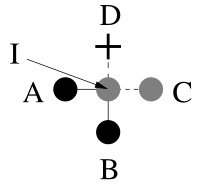
\includegraphics[width=150bp]{figure/closer_points.png}
    \caption{$I$点相邻点}
    \label{closer_points}
\end{figure}

接下来我们看一下快速行进法的算法描述:

初始化
\begin{equation*}
    \label{fmm_init}
    \left\{
    \begin{aligned}
    & t_0 & = & 0 \\
    & A^0 & = & \{I \in Z^2, x_I \notin \Omega\} \\
    & u^0_I = \left\{
        \begin{aligned}
        & 0 & I \in A^0 \\
        & +\infty & I \notin A^0
        \end{aligned}
        \right.
    \end{aligned}
    \right.
\end{equation*}

从第$n$步到第$n+1$步,我们假设$t_n, A^n, u^n$都已知。

首先,我们计算时间的候选值$\widetilde{u}^n_I$,对于每一个$I \in F^n$,找到$\widetilde{u}^n_I$的唯一解:
\begin{equation*}
    \label{uI_unique}
    0 = S_I(\widetilde{u}^n_I, \{u^n_J\}_{J \in V^*(I)}), \mbox{其中} V^*(I) = V(I) \setminus \{I\}
\end{equation*}

然后,取最小的候选值。
\begin{equation*}
    \label{min_tn+1}
    t_{n+1} = \underset{I \in F^n}{\inf} \widetilde{u}^n_I
\end{equation*}

最后,更新点集和各个函数值。新的已知点集为
\begin{equation*}
    \label{new_an+1}
    NA^{n+1} = \{I \in F^n, \widetilde{u}^n_I = t_n\}
\end{equation*}
可得
\begin{equation*}
    \label{new_values}
    \left\{
    \begin{aligned}
    & t_{n+1},\\
    & A^{n+1} & = & A^n \cup NA^{n+1}, \\
    & u^{n+1}_I & = & \left\{
        \begin{aligned}
        & t_{n+1} & I \in NA^n \\
        & u^n_I & \mbox{其他}
        \end{aligned}
        \right.
    \end{aligned}
    \right.
\end{equation*}

算法结束。

\section{增强快速行进法}

